% ============================================================
% IEEE Conference Paper — IEEEtran class
% Title: DDoS Attack Detection Using ResNeXt50-32x4d with MindSpore
% Authors: Abed Al Rida Nehme, Mohamad Al Ghoush, Mohammed Farhat
% Institution: Beirut Arab University (BAU), Lebanon
% Compile: pdflatex -> bibtex -> pdflatex -> pdflatex
% Note: on Overleaf use \bibliographystyle{IEEEtran} (built-in there)
% ============================================================

\documentclass[conference]{IEEEtran}

\IEEEoverridecommandlockouts

\usepackage[T1]{fontenc}
\usepackage[utf8]{inputenc}
\usepackage{cite}
\usepackage{amsmath,amssymb,amsfonts}
\usepackage{graphicx}
\usepackage{xcolor}
\usepackage{booktabs}
\usepackage{array}
\usepackage{tabularx}
\usepackage{multirow}
\usepackage{url}
\usepackage[caption=false,font=footnotesize]{subfig}
\usepackage{tikz}
\usetikzlibrary{positioning, arrows.meta, shapes.geometric}
\usepackage{pgfplots}
\pgfplotsset{compat=1.18}
\usepackage{listings}
\usepackage{ragged2e}
\usepackage{microtype}
\usepackage{silence}
\WarningFilter{latex}{Command \showhyphens has changed}

\lstset{basicstyle=\ttfamily\scriptsize, breaklines=true,
        frame=none, showstringspaces=false}

% Allow extra inter-word stretch to avoid overfull boxes in narrow columns
\setlength{\emergencystretch}{3em}

% Search order for figures
% Local compile: figures resolved via relative paths above
% Overleaf: upload all figures into a "figures/" subfolder in the project root
\graphicspath{{./}{figures/}{../../ict_innovation_overleaf/figures/}{../../research/figures/}}

% ============================================================
\begin{document}

\title{DDoS Attack Detection Using ResNeXt50-32x4d with MindSpore}

\author{
  \IEEEauthorblockN{Abed Al Rida Nehme}
  \IEEEauthorblockA{\textit{Elec.\ \& Computer Engineering}\\
    \textit{Beirut Arab University}\\
    Beirut, Lebanon\\
    202303149@bau.edu.lb}
  \and
  \IEEEauthorblockN{Mohamad Al Ghoush}
  \IEEEauthorblockA{\textit{Elec.\ \& Computer Engineering}\\
    \textit{Beirut Arab University}\\
    Beirut, Lebanon\\
    202300735@bau.edu.lb}
  \and
  \IEEEauthorblockN{Mohammed Farhat}
  \IEEEauthorblockA{\textit{Elec.\ \& Computer Engineering}\\
    \textit{Beirut Arab University}\\
    Beirut, Lebanon\\
    XXXXXXX@bau.edu.lb}
}

\maketitle

% ============================================================
\begin{abstract}
Distributed Denial of Service (DDoS) attacks exploiting the TCP SYN handshake
remain a persistent threat to network availability.
This paper presents \textit{SYNShield}: an end-to-end deep learning pipeline
that converts raw network packet captures (PCAP) into fixed-size $224\times224$
grayscale images and classifies them as DDoS or benign using a
\textbf{ResNeXt-50 (32$\times$4d)} convolutional neural network trained with
\textbf{Huawei MindSpore} and the \textit{mindcv} toolkit.
The primary model is trained on \textbf{0.3\,s time-window} packet images derived
from the public \textbf{CICDDoS2019} benchmark.
On a held-out test set of 1845 samples it achieves \textbf{98.10\%}
accuracy and a macro F1 score of \textbf{0.9375}, with \textbf{100\%} recall on the
DDoS class.
A blind random sample of 270 balanced test images (seed 42) yields
\textbf{98.9\%} accuracy and macro F1 \textbf{0.9889}.
Cross-domain experiments confirm that train/deploy representation alignment is
mandatory; key findings and operational caveats are documented alongside
reproducible evaluation scripts.

\textbf{Keywords:} SYN flood; DDoS detection; packet-to-image; ResNeXt-50;
MindSpore; CICDDoS2019; intrusion detection; deep learning.
\end{abstract}

% ============================================================
\section{Introduction}
\label{sec:intro}

TCP SYN flood attacks exploit the three-way handshake to exhaust server
connection-state resources by sending large volumes of SYN segments without
completing the handshake.
Despite their relative simplicity, SYN floods account for a substantial fraction
of volumetric DDoS incidents observed in operational networks~\cite{sharafaldin2018developing}.
Signature-based and shallow machine-learning intrusion detection systems (IDS)
struggle with obfuscated or novel attack variants, making automated, data-driven
detection an active research challenge.

A compelling direction is the \textit{packet-to-image} paradigm: raw packet bytes
are arranged as two-dimensional pixel matrices and fed into a convolutional neural
network (CNN), allowing the model to learn discriminative spatial structure
without manual feature engineering~\cite{bazzi2020resnet, lotfollahi2020deep}.
Building on this foundation, this paper replaces the ResNet-50 architecture used
in earlier BAU work~\cite{bazzi2020resnet} with \textbf{ResNeXt-50 (32$\times$4d)}—a
grouped-convolution variant offering richer representational capacity at similar
parameter counts~\cite{xie2017aggregated}—and implements the entire training and
inference stack on \textbf{Huawei MindSpore}~\cite{mindspore} with
\textit{mindcv}~\cite{mindcv}.

\textbf{Contributions.}
\begin{itemize}
  \item A reproducible PCAP-to-checkpoint pipeline from CICDDoS2019 zips to
        trained model, including SYN-based heuristic labeling, packet-to-image
        conversion, and class-imbalance-aware training.
  \item A \textbf{0.3\,s time-window} image encoding as the primary training
        representation, with focal-loss~\cite{lin2017focal} training and
        DDoS-F1-oriented early stopping.
  \item Quantitative evaluation including full split metrics, blind inference,
        calibration diagnostics, and a cross-domain mismatch study.
  \item First open, reproducible DDoS image classifier built entirely on
        MindSpore, supporting deployment on CPU and GPU (with an Ascend-compatible
        graph export path).
\end{itemize}

The rest of the paper is organized as follows.
Section~\ref{sec:related} surveys related work.
Section~\ref{sec:method} describes the system design and methodology.
Section~\ref{sec:results} presents experimental results.
Section~\ref{sec:discussion} discusses limitations and operational caveats.
Section~\ref{sec:conclusion} concludes with future directions.

% ============================================================
\section{Related Work}
\label{sec:related}

\subsection{DDoS Detection: Classical and Feature-Based Methods}
Early DDoS detection relied on rule-based thresholds and statistical features
such as SYN/ACK ratios or packet rates~\cite{sharafaldin2018developing}.
While fast and interpretable, these approaches are brittle against rate-varied or
low-and-slow attacks.
Machine learning (ML) on engineered flow features improves adaptability but
requires substantial domain expertise for feature selection and is sensitive to
feature drift.

\subsection{Deep Learning for Network Intrusion Detection}
Deep learning methods have been applied broadly to intrusion detection, spanning
recurrent models for sequential traffic, autoencoders for anomaly scoring
(e.g.,~Kitsune~\cite{mirsky2019kitsune}), and hybrid CNN–RNN architectures
reviewed in~\cite{vinayakumar2019deep}.
SDN-integrated deep learning detectors~\cite{niyaz2016deep} demonstrate
near-real-time capability but depend on controller telemetry not always available
in classical networks.

\subsection{Packet-to-Image Representations}
Lotfollahi et al.~\cite{lotfollahi2020deep} showed that raw byte sequences fed to
CNNs can classify encrypted traffic without decryption.
Bazzi et al.~\cite{bazzi2020resnet} applied this idea specifically to SYN flood
detection on CICDDoS2019~\cite{cicddos2019}, encoding individual packet bytes as
$224\times224$ grayscale images and classifying with ResNet-50~\cite{he2016deep},
achieving strong benchmark accuracy.
Our work extends this line by (i)~upgrading to ResNeXt-50~\cite{xie2017aggregated},
(ii)~using \textit{time-window} aggregation for temporal context,
(iii)~deploying on MindSpore, and (iv)~systematically studying cross-domain
representation transfer.

\subsection{Summary Comparison}
Table~\ref{tab:related} positions this work relative to representative prior
approaches.

\begin{table}[htbp]
\centering
\caption{Qualitative comparison with representative detection approaches.}
\label{tab:related}
\renewcommand{\arraystretch}{1.15}
\begin{tabular}{@{}>{\RaggedRight\arraybackslash}p{1.75cm}
                   >{\RaggedRight\arraybackslash}p{2.45cm}
                   >{\RaggedRight\arraybackslash}p{2.35cm}@{}}
\toprule
\textbf{Method} & \textbf{Strengths} & \textbf{Limitations} \\
\midrule
Rules / thresholds & Fast, explainable & Brittle to novel attacks \\
ML on flow features & Data-adaptive & Feature engineering burden \\
Kitsune~\cite{mirsky2019kitsune} & Unsupervised anomaly & No DDoS-specific supervision \\
ResNet packet-image~\cite{bazzi2020resnet} & Raw-byte patterns; strong CIC results & Single architecture; per-packet only \\
\textbf{This work} & ResNeXt; time-window; MindSpore; full pipeline & Lab dataset; same-domain eval \\
\bottomrule
\end{tabular}
\end{table}

% ============================================================
\section{System Design and Methodology}
\label{sec:method}

\subsection{Dataset}
We use the \textbf{CICDDoS2019} dataset~\cite{cicddos2019} from the Canadian
Institute for Cybersecurity, which contains realistic benign and attack traffic
including multiple SYN flood scenarios captured under controlled laboratory
conditions.
Raw data are provided as PCAP archives and processed through the pipeline
described below.

\subsection{PCAP Labeling}
A lightweight SYN-count heuristic labels each PCAP before image conversion:
any PCAP with more than \textbf{100 TCP SYN packets} is assigned the \textit{DDoS}
class; otherwise it is labeled \textit{normal}.
This threshold was chosen to reflect the high-volume nature of SYN floods
and to avoid false positives from connection-heavy but benign services.
The labeling script (\texttt{classify\_pcap\_syn.py}) performs an early exit
once the threshold is exceeded, making it fast even on large captures.

\subsection{Packet-to-Image Encoding}
For DDoS PCAPs, only TCP SYN packets are extracted (\texttt{--syn-only}) to
isolate the attack signature; for normal PCAPs all packets are used.
Raw packet bytes are arranged sequentially into a 2D array and resized to
$\mathbf{224\times224}$ grayscale pixels using Pillow, following the
methodology in~\cite{bazzi2020resnet}.
During training, grayscale images are replicated to three channels to match the
ImageNet-pretrained normalization expected by the backbone.
Figure~\ref{fig:samples} illustrates example images from each class.

\begin{figure}[htbp]
  \centering
  \subfloat[Normal (benign) traffic]{%
    
\includegraphics[width=0.47\linewidth]{sample_normal.png}%
  }\hfill
  \subfloat[SYN-flood DDoS traffic]{%
    
\includegraphics[width=0.47\linewidth]{sample_ddos.png}%
  }
  \caption{Representative $224\times224$ grayscale packet images from the
           primary 0.3\,s time-window pipeline on CICDDoS2019.}
  \label{fig:samples}
\end{figure}

\subsection{Time-Window Aggregation}
The \textbf{primary model} uses a \textbf{0.3\,s time-window} scheme:
packets captured within a rolling 0.3\,s interval are aggregated into
a single image, providing temporal context across multiple packets within
the window.
The resulting image set is stored under
\path{dataset/images_per_second_window_0p3/} with \texttt{train/},
\texttt{val/}, and \texttt{test/} subdirectories, each containing
\texttt{ddos/} and \texttt{normal/} class folders.
A legacy \textbf{per-packet} configuration (one image per individual packet)
is retained for comparison.

\subsection{Model Architecture}
The classifier is \textbf{ResNeXt-50 (32$\times$4d)}~\cite{xie2017aggregated},
instantiated via \textit{mindcv}~\cite{mindcv} with a two-unit classification
head (DDoS vs.\ normal) and a softmax output layer.
ResNeXt extends ResNet by replacing standard $3\times3$ convolutions with
\textit{grouped} convolutions parameterized by a cardinality $C=32$ and
per-group width $d=4$, which increases representational diversity without
proportionally increasing model size~\cite{xie2017aggregated}.

\subsection{End-to-End Pipeline}
Figure~\ref{fig:pipeline} summarizes the complete flow from raw captures to
inference decision.

\begin{figure}[htbp]
  \centering
  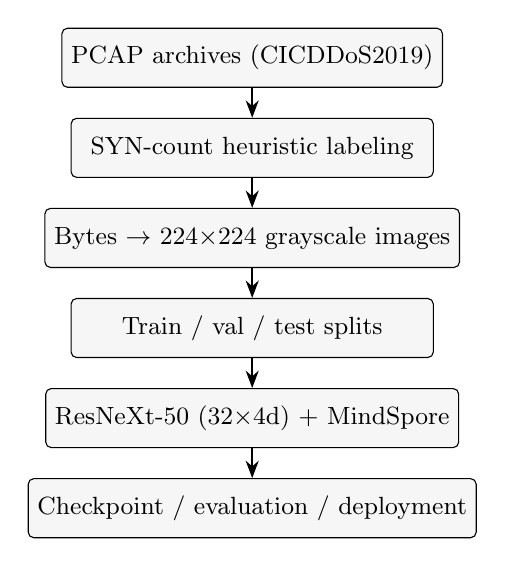
\begin{tikzpicture}[
    node distance=0.38cm and 0.0cm,
    box/.style={rectangle, draw=black, rounded corners=2pt,
      minimum height=0.75cm, minimum width=4.6cm,
      align=center, font=\small, fill=gray!7},
    arr/.style={-{Stealth[length=2.2mm]}, thick}]
    \node[box] (pcap)  {PCAP archives (CICDDoS2019)};
    \node[box, below=of pcap]  (lab)   {SYN-count heuristic labeling};
    \node[box, below=of lab]   (conv)  {Bytes $\rightarrow$ $224{\times}224$ grayscale images};
    \node[box, below=of conv]  (split) {Train / val / test splits};
    \node[box, below=of split] (model) {ResNeXt-50 (32$\times$4d) + MindSpore};
    \node[box, below=of model] (eval)  {Checkpoint / evaluation / deployment};
    \draw[arr] (pcap)  -- (lab);
    \draw[arr] (lab)   -- (conv);
    \draw[arr] (conv)  -- (split);
    \draw[arr] (split) -- (model);
    \draw[arr] (model) -- (eval);
  \end{tikzpicture}
  \caption{End-to-end \textit{SYNShield} pipeline: raw network captures to
           inference decision via packet-image classification.}
  \label{fig:pipeline}
\end{figure}

\subsection{Training Configuration}
Training is implemented in \path{notebook/train_resnext.py} and launched by
\path{scripts/train_resnext_per_second_0p3.sh}.
Table~\ref{tab:hyper} details the primary hyperparameter choices.

\begin{table}[htbp]
\centering
\caption{Primary training hyperparameters (\texttt{per\_second\_0p3\_focal\_v2}).}
\label{tab:hyper}
\renewcommand{\arraystretch}{1.1}
\begin{tabular}{@{}ll@{}}
\toprule
\textbf{Hyperparameter} & \textbf{Value} \\
\midrule
Framework         & Huawei MindSpore 2.6.0 (Graph mode) \\
Backbone          & ResNeXt-50 (32$\times$4d) via mindcv \\
Loss function     & Focal loss~\cite{lin2017focal} ($\gamma{=}2.0$, minority boost $8\times$) \\
Early stopping    & Val DDoS-F1 (\texttt{f1\_ddos}), patience 10 epochs \\
Max epochs        & 40 \\
Batch size        & 32 \\
Optimizer         & Adam (cosine LR schedule) \\
Learning rate     & $5{\times}10^{-4}$ decaying to $10^{-6}$ (1 warm-up epoch) \\
Augmentation (train) & RandomResizedCrop(224), RandomHorizontalFlip \\
Preprocessing (eval) & Resize 256 $\rightarrow$ CenterCrop 224, ImageNet norm. \\
Checkpoint metric & Macro F1 on validation set \\
\bottomrule
\end{tabular}
\end{table}

\textbf{Class imbalance.} The CICDDoS2019 0.3\,s split is heavily skewed toward
normal traffic (1710 normal vs.\ 133 DDoS in validation).
We address this with \textbf{focal loss} combined with an \textbf{8$\times$ minority
boost} on the DDoS class, and use DDoS-class F1 on the validation set as the
early-stopping criterion to prioritize attack recall.

% ============================================================
\section{Experimental Results}
\label{sec:results}

\subsection{Experimental Setup}
All offline evaluations were recorded on \textbf{2026-04-03} using the
\texttt{focal\_v2} primary checkpoint.
Hardware: \textbf{NVIDIA GeForce RTX~3070};
software: MindSpore~2.6.0, mindcv~0.3.0, Python~3.10.12, CUDA~11.6.
The one-shot driver is \path{scripts/run_all_eval_0p3.sh};
fixed seed~42 ensures reproducibility.

\subsection{Primary Model: 0.3\,s Time-Window}
Table~\ref{tab:mainresults} presents overall accuracy, macro F1, weighted F1,
and balanced accuracy on the validation and test splits.

\begin{table}[htbp]
\centering
\caption{Overall metrics for the primary 0.3\,s window model.}
\label{tab:mainresults}
\renewcommand{\arraystretch}{1.1}
\begin{tabular}{@{}lrrrr@{}}
\toprule
\textbf{Split} & \textbf{$N$} & \textbf{Acc.} & \textbf{Macro F1} & \textbf{Bal.\ Acc.} \\
\midrule
Validation & 1842 & 98.21\% & 0.9399 & 0.990 \\
Test       & 1845 & 98.10\% & 0.9375 & 0.990 \\
\bottomrule
\end{tabular}
\end{table}

\subsection{Confusion Matrices}
Table~\ref{tab:confusion} provides the raw confusion counts for both splits.
Notably, the model achieves \textbf{zero missed DDoS samples} (false negatives)
on both validation and test, at the cost of 33 and 35 false positives,
respectively.

\begin{table}[htbp]
\centering
\caption{Confusion matrices (rows = true class, cols = predicted class).}
\label{tab:confusion}
\renewcommand{\arraystretch}{1.1}
\begin{tabular}{@{}lccrcc@{}}
\toprule
 & \multicolumn{2}{c}{\textbf{Validation}} && \multicolumn{2}{c}{\textbf{Test}} \\
\cmidrule{2-3}\cmidrule{5-6}
\textbf{True\,\textbackslash\,Pred} & DDoS & Normal && DDoS & Normal \\
\midrule
DDoS   & \textbf{133} & 0  && \textbf{135} & 0  \\
Normal & 33  & \textbf{1676} && 35  & \textbf{1675} \\
\bottomrule
\end{tabular}
\end{table}

\subsection{Per-Class Precision, Recall, and F1}
Table~\ref{tab:perclass} shows per-class metrics derived from the confusion
matrices.
The DDoS class achieves \textbf{recall = 1.000} (no missed attacks) in both
splits, which is the operationally critical metric for a security detector.

\begin{table}[htbp]
\centering
\caption{Per-class precision, recall, and F1 on validation and test.}
\label{tab:perclass}
\renewcommand{\arraystretch}{1.1}
\begin{tabular}{@{}lrrrrrr@{}}
\toprule
 & \multicolumn{3}{c}{\textbf{Validation}} & \multicolumn{3}{c}{\textbf{Test}} \\
\cmidrule{2-4}\cmidrule{5-7}
\textbf{Class} & Prec. & Rec. & F1 & Prec. & Rec. & F1 \\
\midrule
DDoS   & 0.801 & 1.000 & 0.890 & 0.794 & 1.000 & 0.885 \\
Normal & 1.000 & 0.981 & 0.990 & 1.000 & 0.980 & 0.990 \\
\midrule
Macro  & \multicolumn{3}{c}{0.940} & \multicolumn{3}{c}{0.937} \\
\bottomrule
\end{tabular}
\end{table}

Figure~\ref{fig:barchart} visualizes the per-class precision, recall, and F1
on the test split.

\begin{figure}[htbp]
  \centering
  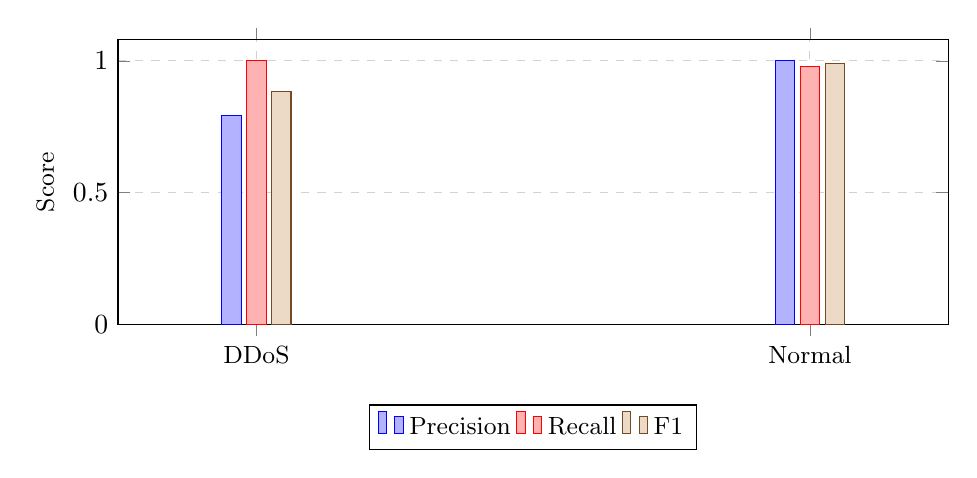
\begin{tikzpicture}
    \begin{axis}[
      ybar, bar width=7pt, ymin=0, ymax=1.08,
      ylabel={Score}, ylabel style={font=\small},
      symbolic x coords={DDoS, Normal},
      xtick=data, x tick label style={font=\small},
      legend style={font=\small, at={(0.5,-0.28)}, anchor=north,
                    legend columns=3},
      width=\linewidth, height=5.2cm,
      enlarge x limits=0.25,
      grid=major, major grid style={dashed,gray!35},
    ]
      \addplot coordinates {(DDoS,0.794) (Normal,1.000)};
      \addplot coordinates {(DDoS,1.000) (Normal,0.980)};
      \addplot coordinates {(DDoS,0.885) (Normal,0.990)};
      \legend{Precision, Recall, F1}
    \end{axis}
  \end{tikzpicture}
  \caption{Per-class precision, recall, and F1 on the test split.
           DDoS recall = 1.000 reflects zero missed attacks.}
  \label{fig:barchart}
\end{figure}

\subsection{Blind Test}
To reduce evaluation bias from label order, \path{scripts/blind_test_random.py}
draws a balanced random sample from the test split (model receives images only,
no label information).
With the maximum balanced sample of \textbf{270 images} (135 DDoS + 135 normal,
seed 42), the model correctly classifies 267 of 270 images:

\begin{center}
\begin{tabular}{@{}lrr@{}}
\toprule
\textbf{True\textbackslash Pred} & DDoS & Normal \\
\midrule
DDoS   & 135 & 0 \\
Normal & 3   & 132 \\
\midrule
Accuracy & \multicolumn{2}{c}{\textbf{98.9\%}} \\
Macro F1 & \multicolumn{2}{c}{\textbf{0.9889}} \\
\bottomrule
\end{tabular}
\end{center}

\subsection{ROC, Precision--Recall, and Calibration}
Figure~\ref{fig:rocpr} shows the ROC and precision--recall curves on the
test split (generated by \path{scripts/eval_roc_pr_calibration.py}).
The calibration diagnostic yields a test \textbf{Expected Calibration
Error (ECE) $\approx$ 0.074} and a heuristic max-F1 threshold of
$\approx 0.87$ on the DDoS softmax probability (Fig.~\ref{fig:diag}).

\begin{figure}[htbp]
  \centering
  \subfloat[ROC curve]{%
    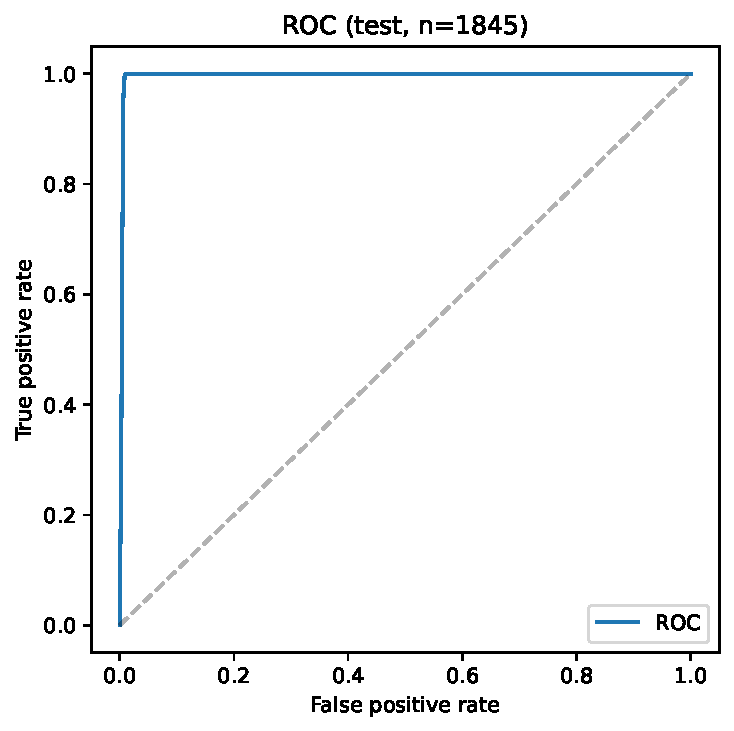
\includegraphics[width=0.47\linewidth]{roc_test.pdf}%
  }\hfill
  \subfloat[Precision--recall curve]{%
    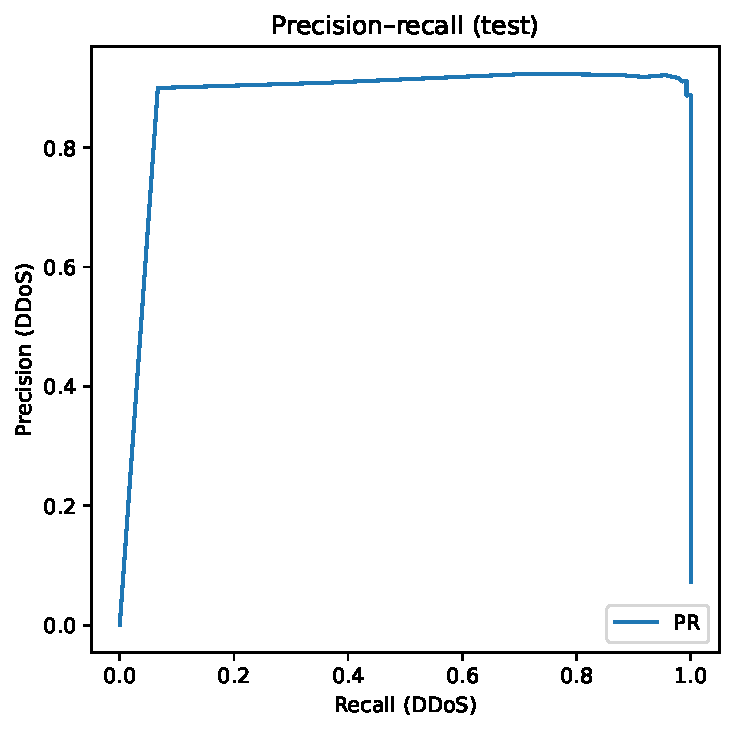
\includegraphics[width=0.47\linewidth]{pr_test.pdf}%
  }
  \caption{ROC and precision--recall curves for the primary 0.3\,s model
           on the test split (via \texttt{run\_all\_paper\_figures.sh}).}
  \label{fig:rocpr}
\end{figure}

\begin{figure}[htbp]
  \centering
  \subfloat[Confusion matrix heatmap]{%
    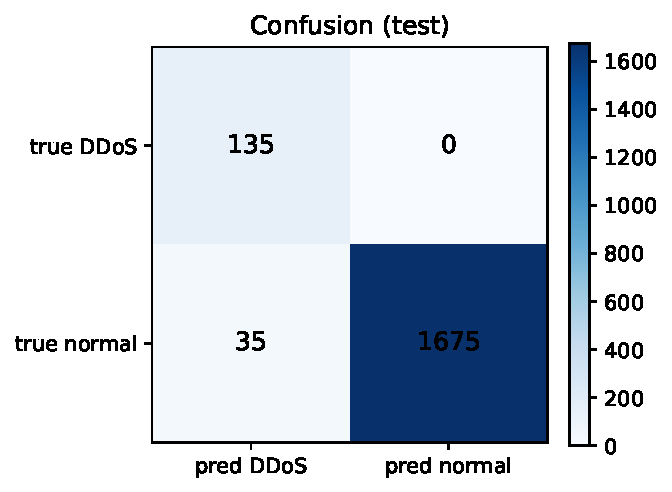
\includegraphics[width=0.47\linewidth]{confusion_heatmap_test.pdf}%
  }\hfill
  \subfloat[Threshold vs.\ F1 sweep]{%
    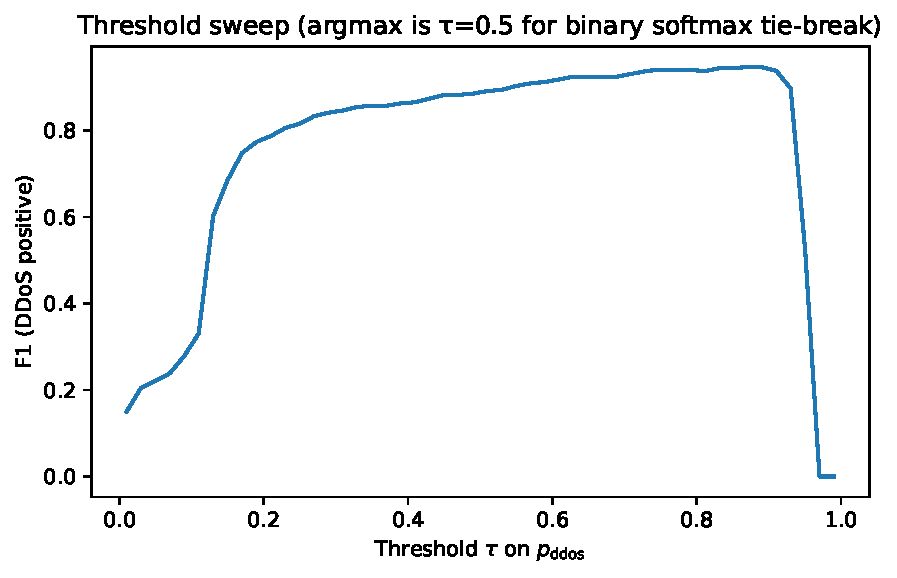
\includegraphics[width=0.47\linewidth]{threshold_f1_test.pdf}%
  }
  \caption{Test-split diagnostics: confusion heatmap (left) and F1 score
           as a function of the DDoS probability threshold (right). The
           heuristic max-F1 threshold is $\approx 0.87$.}
  \label{fig:diag}
\end{figure}

\subsection{Comparison with Baselines}
Table~\ref{tab:baseline} contrasts the primary model with a trivial majority
classifier and the legacy per-packet configuration.

\begin{table}[htbp]
\centering
\caption{Performance comparison across configurations on respective test sets.}
\label{tab:baseline}
\renewcommand{\arraystretch}{1.1}
\begin{tabular}{@{}>{\RaggedRight\arraybackslash}p{3.2cm}rrc@{}}
\toprule
\textbf{Configuration} & \textbf{$N$} & \textbf{Acc.} & \textbf{Macro F1} \\
\midrule
Always predict Normal & 1845 & 92.7\% & 0.481 \\
Per-packet ckpt\,$^\dagger$ on 0.3\,s test (cross-domain) & 1845 & 89.9\% & 0.473 \\
Per-packet ckpt\,$^\dagger$ on per-packet test & 19\,300 & 98.8\% & 0.497 \\
Per-packet ckpt\,$^\dagger$ blind test & 3000 & 99.9\% & 0.9993 \\
\textbf{Ours (0.3\,s, primary)} & \textbf{1845} & \textbf{98.10\%} & \textbf{0.9375} \\
\bottomrule
\multicolumn{4}{@{}l}{\scriptsize $^\dagger$\texttt{model/resnext50\_32x4d\_best.ckpt}} \\
\end{tabular}
\end{table}

The majority-class baseline achieves 92.7\% accuracy due to class imbalance,
which confirms that accuracy alone is insufficient for security evaluation.
The macro F1 of the primary model (0.9375) far exceeds the baseline (0.481),
demonstrating meaningful attack detection beyond statistical luck.

% ============================================================
\section{Discussion}
\label{sec:discussion}

\subsection{Cross-Domain Representation Mismatch}
A critical finding is that the two image representations
(per-packet vs.\ 0.3\,s time-window) are \textbf{not interchangeable} without
retraining.
When the 0.3\,s checkpoint is applied to per-packet test images, macro F1 drops
to 0.497 with argmax never predicting DDoS (19\,300 samples; 2026-04-03 run).
Symmetrically, the per-packet checkpoint applied to the 0.3\,s test set yields
macro F1 of 0.473 with zero DDoS recall.
This finding underlines a fundamental requirement: \textbf{deployment must use
the same image construction as training}.

\subsection{Operational Considerations}
The live inference service (\texttt{run\_pipeline.py}) processes per-packet
images within rotating 0.3\,s PCAP windows. Each window logs a prediction
$\mathit{pred} \in \{\text{ddos}, \text{normal}\}$ and the DDoS probability
$p_\text{ddos}$.
On public interfaces, Internet background traffic—scans, probing, heterogeneous
protocols—may differ substantially from CICDDoS2019 training traffic, causing
elevated false-positive rates.
Consequently, $p_\text{ddos}$ values from the deployed model represent
\textbf{classifier suspicion}, not confirmed incidents.
Operational use cases should layer threshold tuning on $p_\text{ddos}$,
consecutive-window voting, or hybrid rules before triggering automated
responses.

\subsection{Label-Quality Validation and Cross-Day Generalization}
\label{sec:labelvalidation}
The primary results above rely on the SYN-count heuristic of
Section~\ref{sec:method}. To test whether that heuristic limits
generalization, we built a second labeling pipeline that clusters
per-window flow features (unsupervised $k$-means) and accepts a cluster
split as the attack label only if its mean SYN ratio exceeds the other
cluster's (a flood-signature gate), falling back to schedule-based labels
otherwise. We paired this with a \textit{FlowPic}-style
encoding~\cite{shapira2019flowpic}: each 0.3\,s window becomes a
$64\times64$ packet-size$\times$arrival-time histogram, avoiding the
natural-image assumptions of the byte-dump encoding above.

To stress-test generalization beyond the same-domain split used
elsewhere in this paper, we held out an \textbf{entire attack day}
(\texttt{01-12-2018}) as test and trained only on the other attack day
(\texttt{03-11-2018}) plus normal-only captures --- a cross-day test, not
just unseen windows from an attack the model saw part of. The resulting
model reached validation $\mathit{f1\_ddos}=0.866$, but held-out
cross-day test $\mathit{f1\_ddos}$ dropped to \textbf{0.419}. We
cross-referenced the flagged false positives against CICFlowMeter's
official per-flow \texttt{Label} column --- independent of both our
derived labels and the model's own predictions --- and confirmed that
\textbf{86 of 2{,}071} flagged windows (4\%) are provably mislabeled by
the schedule-boundary heuristic; relabeling only those raises test
$\mathit{f1\_ddos}$ to \textbf{0.453} (Table~\ref{tab:gapfix}). Feature
and visual inspection of the remaining, unverifiable false positives
shows they resemble genuine (if busier-than-typical) normal traffic
rather than disguised attack traffic, so we report this as a real,
only partially label-driven cross-day generalization gap rather than
overstate it as a pure labeling artifact.

\begin{table}[htbp]
\centering
\caption{Cross-day test metrics before/after relabeling confirmed mislabels.}
\label{tab:gapfix}
\renewcommand{\arraystretch}{1.1}
\begin{tabular}{@{}lrr@{}}
\toprule
\textbf{Metric} & \textbf{Raw} & \textbf{Corrected (86 relabeled)} \\
\midrule
Accuracy      & 0.7805 & 0.7889 \\
DDoS F1       & 0.419  & 0.453  \\
\bottomrule
\end{tabular}
\end{table}

\subsection{Limitations}
\begin{itemize}
  \item Evaluation is \textbf{same-domain} (train and test from CICDDoS2019);
        generalization to other datasets or enterprise traffic is not validated.
  \item The SYN-count labeling heuristic may mislabel PCAPs containing
        connection-heavy benign services; Section~\ref{sec:labelvalidation}
        found this accounts for a confirmed 4\% of cross-day test false
        positives, with the remaining gap attributable to genuine
        generalization difficulty rather than mislabeling.
  \item The system covers only TCP SYN floods; UDP amplification, HTTP floods,
        and application-layer attacks are out of scope.
  \item Adversarial crafting of packet bytes to evade the image classifier
        is not evaluated.
\end{itemize}

% ============================================================
\section{Conclusion and Future Work}
\label{sec:conclusion}

We presented \textit{SYNShield}, an end-to-end deep learning pipeline for
detecting SYN flood DDoS attacks by classifying 0.3\,s time-window packet
images with a ResNeXt-50 model trained on Huawei MindSpore.
The primary model achieves \textbf{98.10\%} test accuracy, \textbf{0.9375}
macro F1, and \textbf{100\% recall on the DDoS class} with zero missed attacks.
A blind evaluation on 270 balanced samples confirms strong performance at 98.9\%
accuracy and macro F1 of 0.9889.
Cross-domain experiments reveal that representation alignment between training
and deployment is non-negotiable; operational deployments that violate this
constraint exhibit near-random DDoS detection.

\textbf{Future work} includes:
(1)~validation on additional DDoS families (UDP, HTTP-flood) and out-of-distribution
packet traces;
(2)~systematic comparison of window lengths (0.3\,s, 1\,s, 5\,s) and
dual-view fusion (SYN-only vs.\ all-packets);
(3)~hardware export to Huawei Ascend NPU for edge deployment;
(4)~calibrated alert strategies (thresholded $p_\text{ddos}$, temporal
smoothing) to reduce false positives on live Internet traffic;
(5)~adversarial robustness evaluation and domain adaptation under concept drift.

% ============================================================
\section*{Acknowledgment}
The authors thank Eng.\ Mustafa Bizri (Beirut Arab University) for project
supervision and guidance throughout this work.
They also thank the Canadian Institute for Cybersecurity for releasing the
CICDDoS2019 dataset, and the Huawei MindSpore and \textit{mindcv} teams
for the open-source deep learning framework used in all experiments.

% ============================================================
% IEEEtran native last-page column balancer: insert a column break
% before this reference number so both columns end at the same height.
% Adjust the number if the reference count changes.
\IEEEtriggeratref{8}
\bibliographystyle{unsrt}
\bibliography{references}

\end{document}
